\documentclass[12pt]{article}
\usepackage{xcolor}
\usepackage{graphicx}
\usepackage{rotating}
\usepackage{lscape}
\usepackage{booktabs}
\usepackage{comment}
\usepackage{listings}
\usepackage{multicol,multirow}
\usepackage[top=1in, bottom=1in, left=1.25in, right=1.0in]{geometry}
\usepackage{hyperref}
\usepackage{longtable}


% A few paragraph formatting parameters:
\parskip = 6pt
\parindent = 0.0in

% Set up the 'listings' package:
\lstdefinestyle{custombash}{
 language=bash, 
 columns=fullflexible, 
 breaklines=true, 
 basicstyle=\ttfamily\footnotesize, 
 numbers=left, 
 numbersep=5pt,
 commentstyle=\itshape\color{mygreen},
 keywordstyle=\bfseries\color{blue},
 numberstyle=\tiny\ttfamily\color{black}, 
 stringstyle=\color{brown},
 otherkeywords={DISPLAY,EXPORT, IMAGE, MONOCHROME, RIPUP, SET, COLOR_LAYER},
 frame=single]
}
\lstset{style=custombash}

% Set some parameters for the graphics:
\DeclareGraphicsExtensions{.pdf,.png,.jpg,.jpeg}
\graphicspath{{./}{../}{./images/}}

% The default "BLUE" for the web links isn't much to my liking. 
\definecolor{webblue}{rgb}{0,0,0.75}
\definecolor{mygreen}{rgb}{0,0.6,0}
\definecolor{gray60}{gray}{0.6}

% Some nice, well-worn shortcuts:
\newcommand{\+}{\item}		% easier than typing \item a lot
%\setlength{\parindent}{0in}	% easier than putting \noindent at every paragraph
\newcommand{\bi}{\begin{itemize}}
\newcommand{\ei}{\end{itemize}}
\newcommand{\bd}{\begin{description}}
\newcommand{\ed}{\end{description}}
\newcommand{\be}{\begin{enumerate}}
\newcommand{\ee}{\end{enumerate}}
\newcommand{\rr}{\raggedright}

% some table formatting shortcuts:
\renewcommand{\thefootnote}{\fnsymbol{footnote}}
\newcommand{\sep}{1mm}
\newcommand{\negsep}{-3mm}
\newcommand{\thisscale}{1.6}
\newcommand{\silkscale}{1.0}
\newcommand{\tabitem}{~~\llap{\textbullet}~~}

% Names of the layout graphics files, so nobody has to go looking for them
\newcommand{\colorimagename}{colorlayout.png}
\newcommand{\twolayermonochrome}{whiteboardlayout.png}
\newcommand{\topmonochrome}{toplayout.png}
\newcommand{\bottommonochrome}{bottomlayout.png}
\newcommand{\bottomsilk}{bottomsilk.png}
\newcommand{\topsilk}{topsilk.png}
\newcommand{\boarddimensions}{dimensions.png}

\newcommand{\revision}{1.0}

% A key for optional output:
\newif\ifkey
\keyfalse
% Uncommenting \keytrue would set the "key" variable to TRUE:
\keytrue



\begin{document}
\thispagestyle{empty}
\begin{center}
\begin{Huge}
Atari Punk Console\\
\end{Huge}
\bigskip
\begin{Large}
\ifkey
Assembly, Testing, and Designer's Guide\\
\else
Assembly and Testing Guide\\
\fi

\end{Large}
\bigskip
Board version \revision\\
Guide version 1.1\\
Jesse Hamner\\
March 2017\\
\vspace{0.2in}


\end{center}

\tableofcontents

\vfill 

\begin{center}
\begin{tabular}{c p{1.0in} c}

\includegraphics[scale=0.25]{UNTLibLogoStacked.png} & & 
\includegraphics[scale=0.185]{FactoryBWlogotrimmed.png} \\
\end{tabular}

\emph{Originally developed in collaboration with the UNT Libraries.}
\end{center}

\newpage

\section{Introduction}

In 1983, or some time before that, {\color{webblue}\href{http://www.forrestmims.org}{Forrest Mims III}}, a long-time participant in the electronics, hobbyist, and atmospheric science communities, designed the ``Stepped Tone Generator" using the wildly popular and hugely versatile {\color{webblue}\href{https://en.wikipedia.org/wiki/555_timer_IC}{555 timer integrated circuit}}. He published the design in a Radio Shack (Tandy Corp) book of projects\footnote{Mims, Forrest M., III. 1984. \emph{Engineers's Mini-notebook: 555 Timer IC Projects.} Fort Worth, Texas: Radio Shack.}, and then again in the 1992 \emph{Engineer's Mini-Notebook}\footnote{Mims, Forrest M., III. 1992. \emph{Engineer's Mini-Notebook}. 3\textsuperscript{rd} edition. Fort Worth, Texas: Radio Shack.}.

I was unable to find an example of this board that presented a simple design, an easy soldering task, but also an easy path to customization. People who are getting in to electronics, soldering, and/or ``making" may want a few easy ``wins" for their first few projects, and the ``{\color{webblue}\href{https://en.wikipedia.org/wiki/Atari_Punk_Console}{Atari Punk Console}}", as it has become known, is a simple circuit with a modest amount of expandability. 

I have re-implemented the design with the intent to provide a series of stepping stones from novice to an intermediate ``maker." Maker spaces like UNT's Factory provide a range of tools to end users, but like many tools, learning to use them can be a challenge. Here again, this design of the APC is up to the task. With easy alignment notches and a downloadable reference design for a 3D-printed case, users can learn to solder, solder the APC, and print a case for it, without facing serious hurdles. 

This project and its ancillary pieces allow novices to gain experience in several aspects of hobbyist making, while not facing the full force of electrical or industrial engineering. Put another way: one should not be required to learn typesetting in order to print a Microsoft Word document; neither should one be required to understand G-Code or STL files in order to produce a working and fun electronics project.

This guide provides graphical and instructional information about the assembly of this version of the ``Stepped Tone Generator". Please read this guide all the way through before beginning any work on the boards. 


%%%%%%%%%%%%%%%%%%%

\subsection*{Legal}

This document is intended to assist in the assembly of a circuit board project that synthesizes sound waves. This document comes with ABSOLUTELY NO WARRANTY. This document is released under the Creative Commons Attribution-ShareAlike  (CC BY-SA) license version 4.0. For more, see {\color{webblue}\href{https://creativecommons.org/licenses/}{creativecommons.org}}.
\begin{center}

\includegraphics[scale=1.0]{by-sa.png}
\end{center}

%%%%%%%%%%%%%%%%%%%


\section{Best Practices}
\bi
\+ Use static ground during soldering; these components can be easily damaged by static electricity
\+ Use thin (perhaps 0.032-inch or 0.8mm) solder for through-hole components
\+ Use a good quality soldering iron % or hot air rework station
\+ Clean the tip often on the brass scrubber
\+ Re-tin the tip often
\+ Lifting PCB pads and traces is quite possible without much effort---watch the iron temperature, and don't apply heat for more than ten seconds per soldered pin 
\+ Don't buy or use low-quality solder, leaded or not; it gets gummy and is more or less impossible to remove without thermal damage to your components. Use name-brand solder, like {\color{webblue}\href{http://www.kester.com}{Kester}}
\+ Masking tape may be helpful to hold pin headers in place while soldering the underside
\+ Tweezers or small pliers are useful (but not necessary) for placement of the SMD component
\ei


\section{Useful Equipment For Testing}
\bi
\+ A 9V battery
\+ A 6V to 13.8V DC power source, capable of providing at least 300 milliamps of current
\+ A multimeter
\+ A stereo magnifier, an inspection loupe, and/or a USB microscope
\+ A third hand or PCB vise
\+ A set of headphones or a powered speaker
\ei


\section{Assembly Order}

\begin{itemize}
\+ Discrete resistors
\+ Diodes (note the orientation!)
\+ Disc capacitors
\+ Electrolytic (aluminum, polarized) capacitor(s)
\+ 2- and 3-pin headers
\+ LED (note the orientation!)
\+ 8-pin integrated circuit sockets (note the orientation!)
\+ DC power jack
\+ 9V battery cradle
\+ SMD headphone jack (see text)
\+ Variable resistors (potentiometers / rheostats)
\+ Switch
\end{itemize}

After the sockets are installed, consider the orientation of the 555 timers and press them completely into the sockets. It may be helpful to line up four pins on one side with the socket connector, insert them about 1mm, then gently press the opposite side pins inward until they can also be fit into the socket. 

When soldering the stereo jack, heat a large pad on the PCB and melt a little solder onto it. Align the jack and hold it in place (the tab will be on top of the now-tinned PCB pad) with pliers, tweezers, or whatever you have. Hold the soldering iron tip on top of the tab, or touching both the pad and the tab, and the heat will eventually melt the solder and bond the tab to the board. If you have correctly aligned the jack, the other tabs and pads will be easy to solder. If not, re-melt the solder until you can get the jack to align properly. It may be helpful to press down with the tweezers or pliers (even clamping the board and the jack together with them). You don't want the tab to ``float'' up on the solder blob. 

\section{Hardware Testing}

\bi
\+ Turn the switch to `off'
\+ Install a 9V battery in the battery carrier
\+ Using a multimeter, check the voltage at the output (left, on this board) terminal of diodes D1 and D2
\+ Turn the switch to `on' and check the power LED indicator
\+ If the LED does not illuminate, use a multimeter to confirm that there is at least 6 volts available at the LED positive terminal

\+ Set all the knobs to the middle
\+ plug in the headphones and check for sound

\ei

\clearpage

\section{Board Layout Images}

The next section includes images of the board design and layout for reference during the soldering and testing process. 

\begin{figure}[hb!]
\begin{center}
\includegraphics[scale=\thisscale]{\colorimagename}
\end{center}

\caption{Color image unsuitable for monochrome printing. Both layers visible. Red traces are on the top layer, and blue traces are on the bottom layer. As would be expected if the board was transparent, all components on the bottom (although there are none for this board), and text, are reversed.}
\end{figure}


\begin{figure}
\begin{center}

\includegraphics[scale=\thisscale]{\twolayermonochrome}

\end{center}

\caption{Both layers visible. As would be expected if you could see through the board, elements on the bottom such as printed text are reversed. For this board, \emph{all components, headers, jacks, and connectors should be mounted on the top layer}, and soldered from the underside.}
\end{figure}

\newpage

\begin{figure}
\begin{center}
\includegraphics[scale=1.1]{\topmonochrome}
\end{center}
\caption{Top layer only. Some larger component outlines are shown in gray, as are two alignment notches in the board.}
\end{figure}


\begin{figure}
\begin{center}
\includegraphics[scale=1.1]{\bottommonochrome}
\end{center}
\caption{Bottom layer only. \textbf{Important:} no jacks or headers should be soldered facing ``down" (that is, with the business end of the component on the underside). Note the alignment notches are reversed; this perspective is viewed from the bottom, not through the top of the board.}
\end{figure}


\newpage

\begin{figure}
\begin{center}
\begin{tabular}{cc}

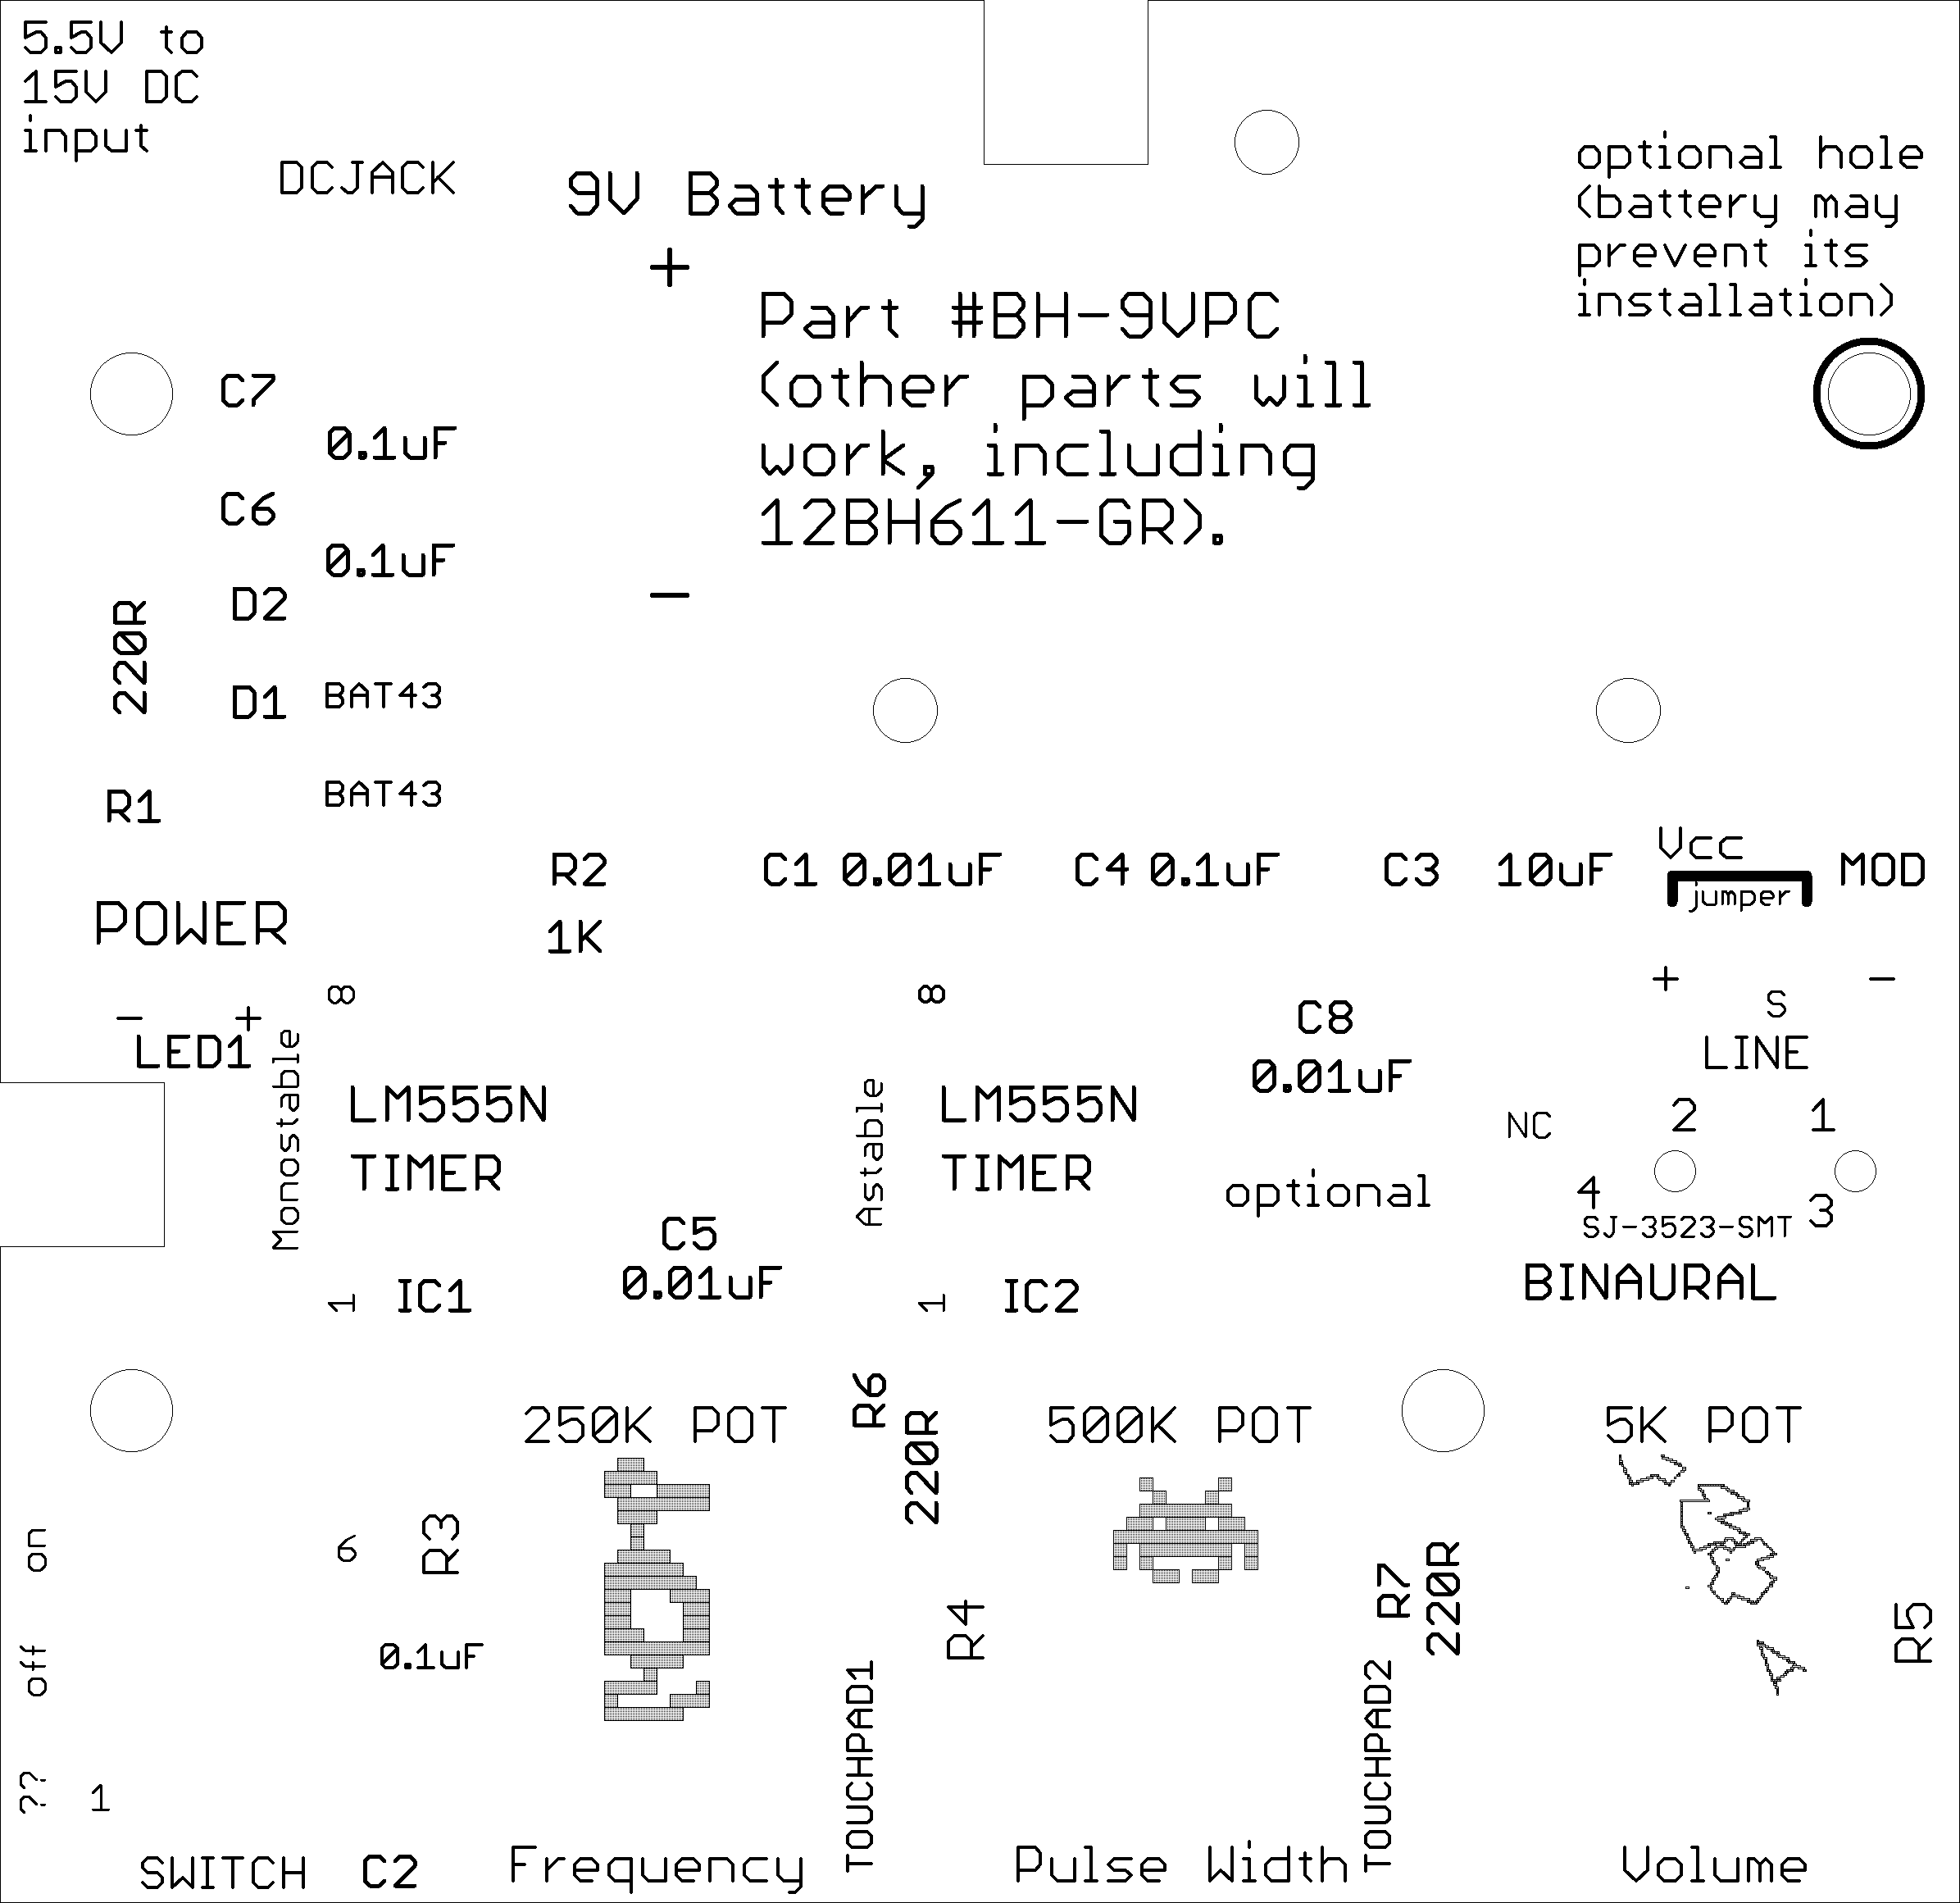
\includegraphics[scale=\silkscale]{\topsilk}

&

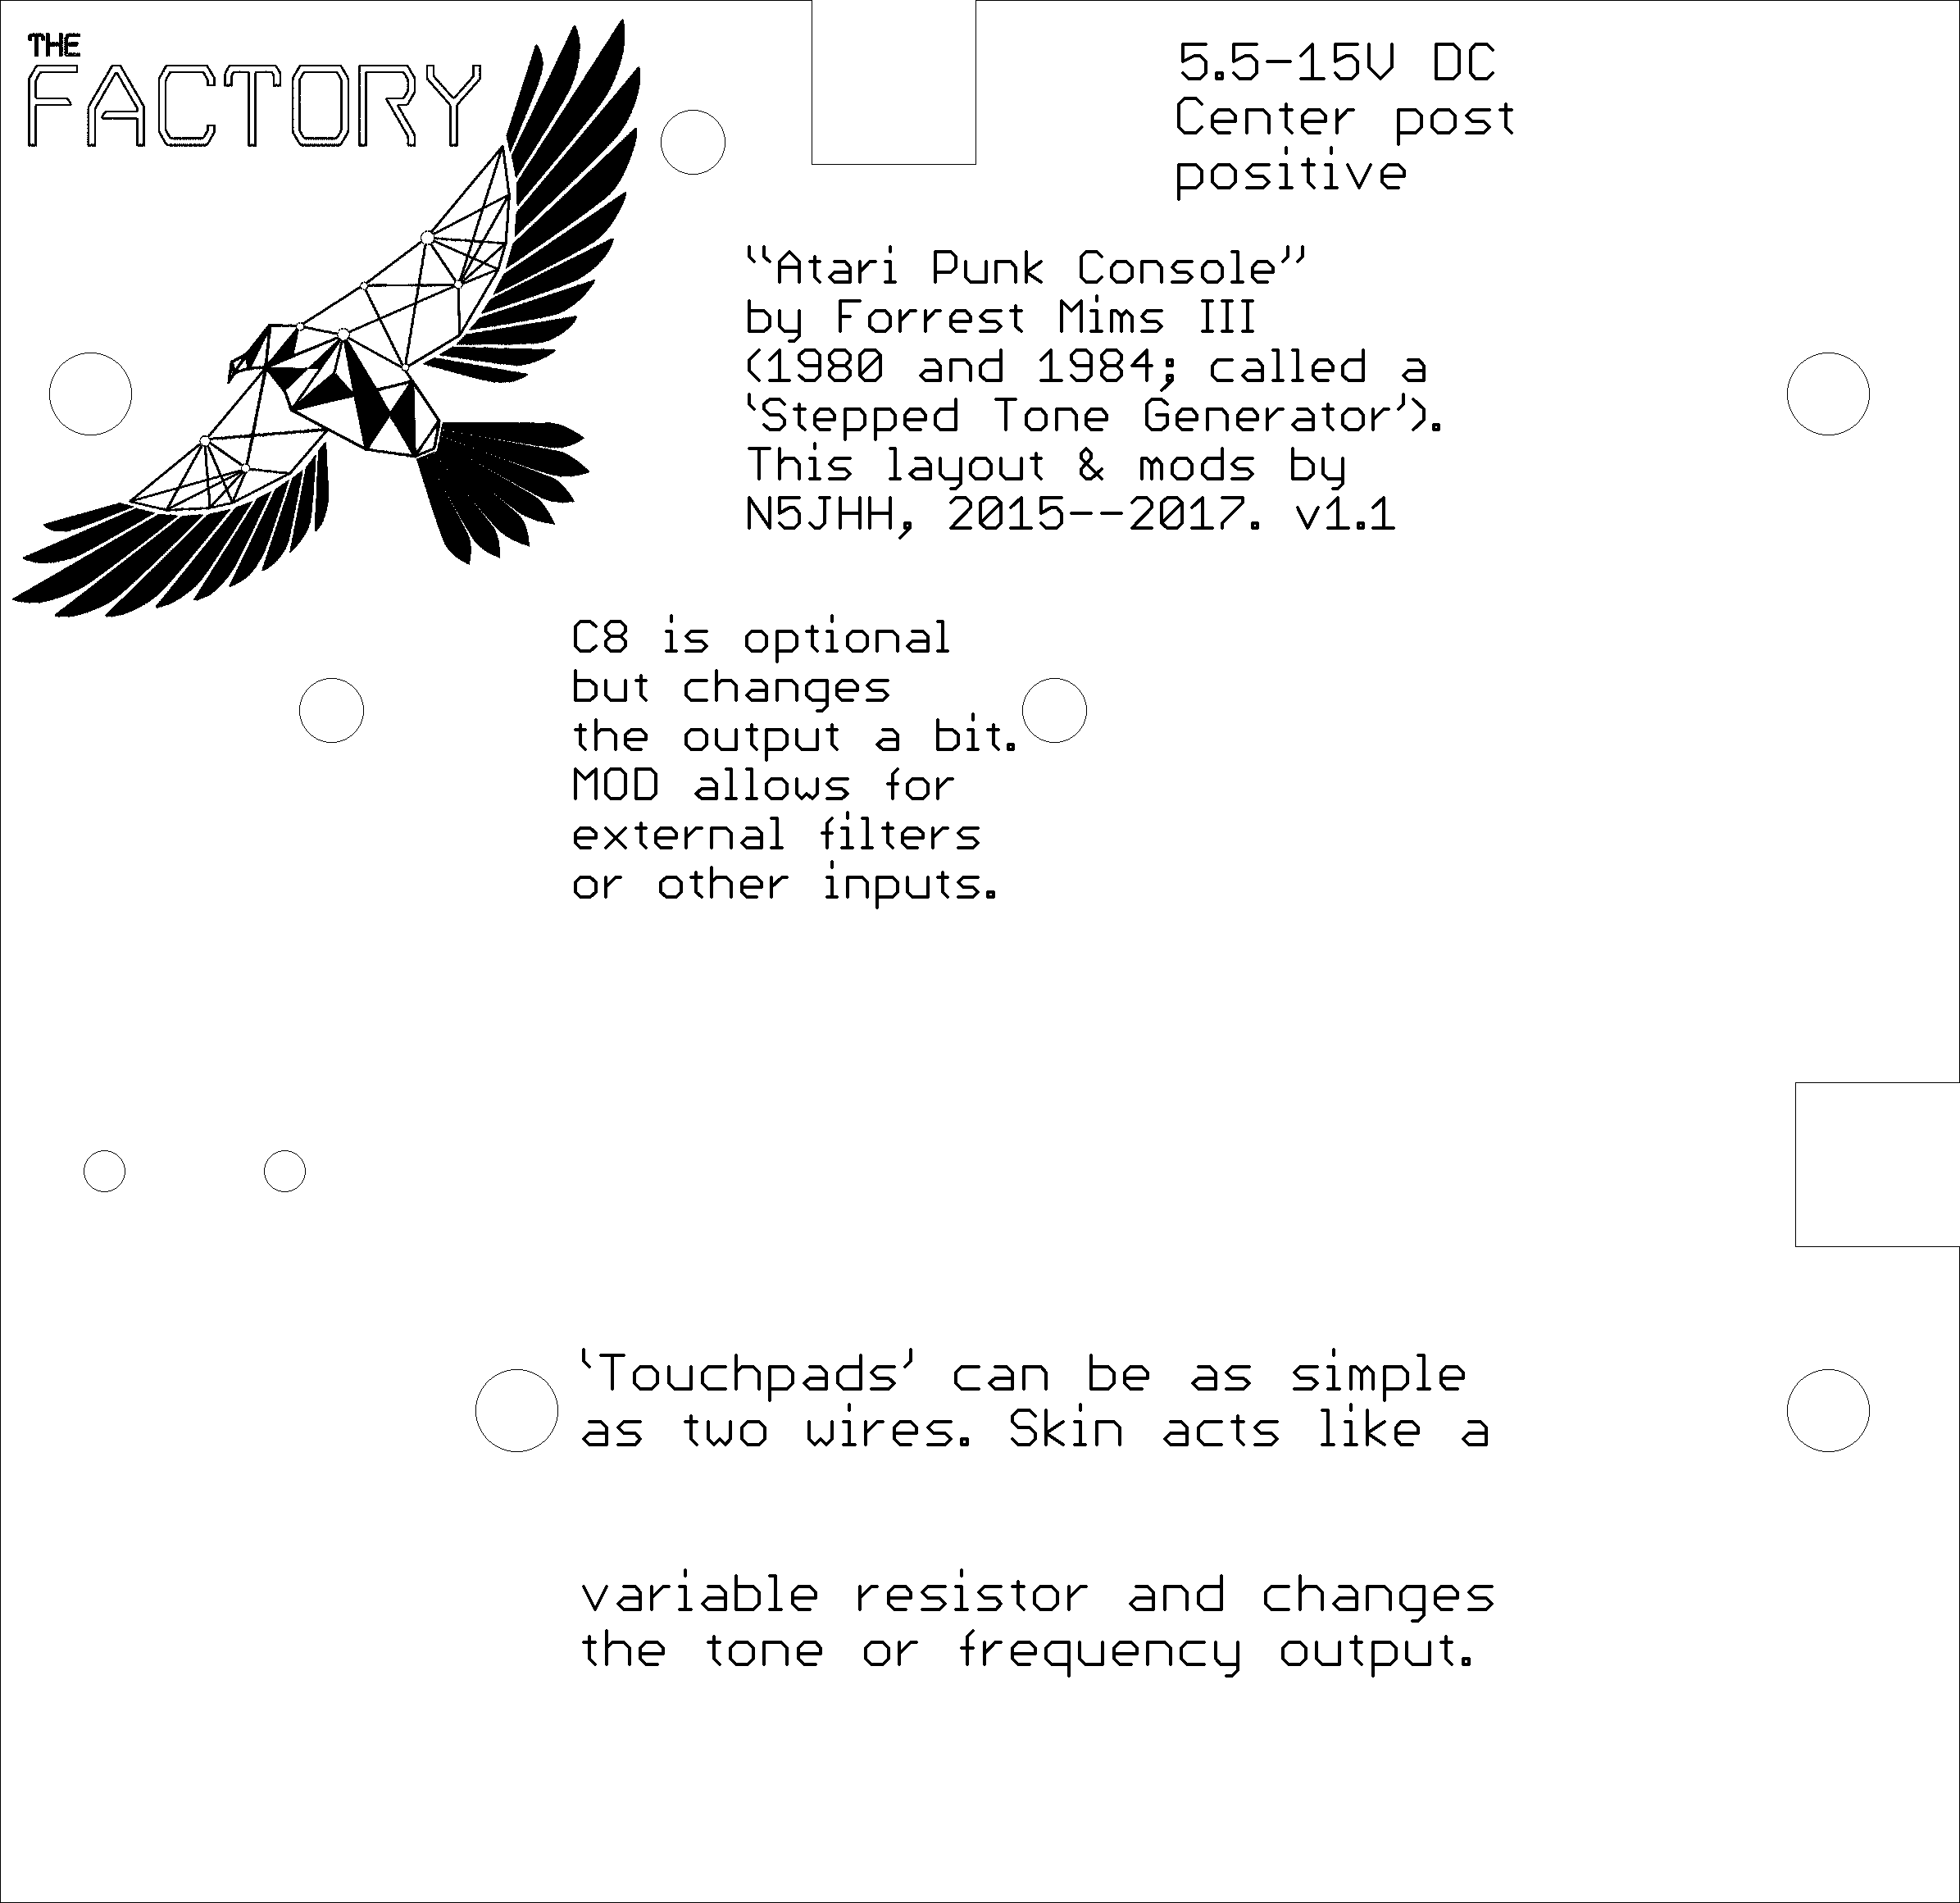
\includegraphics[scale=\silkscale]{\bottomsilk}

\\

\end{tabular}

\end{center}
\caption{Silkscreens for top and bottom of the board. On the top silkscreen, note that the 8-bit Atari and Taito characters will be hidden under the rotary potentiometers once installed. From left to right: a dragon from the Atari 2600 \emph{Adventure} game; a Taito Space Invader; and a screen from \emph{Asteroids}. On the bottom silkscreen: note optional modification information and the Factory logo, copyright UNT Libraries.}
\end{figure}

\begin{figure}
\begin{center}
\includegraphics[scale=1.0]{\boarddimensions}
\end{center}
\caption{Board dimensions, should you want to design an enclosure for it. The three 2mm holes in the battery cradle could be attached to the underside of the enclosure with machine screws and nuts, but all fasteners must be flush with top surface of the cradle, meaning the underside of the enclosure would need recessed pockets for the nuts, or else rubberized feet that were taller than the portion of the fasteners that protrude through the bottom of the enclosure. It is also possible to create standoffs \emph{within} the case that provide underside clearance for fasteners such that the fasteners do not have exposed surfaces outside the case, at the slight expense of a taller overall case.}
\end{figure}




\clearpage 
\section{Device Schematic}

Although not required to successfully assemble and use the Stepped Tone Generator, some may find the schematic useful or interesting. There are also many schematics of similar implementations of Forrest Mims's work online. This implementation stays very close to the original, with a few small additions like the touchpad headers and the optional capacitors, that can be ignored if desired. I varied a few of the other components based on experience. To create this image, from the schematic pane, type (no quotes!)

\verb|EXPORT IMAGE $HOME/some/useful/path/APCschematic.png 800|

\bigskip

\begin{figure}[hb!]
\begin{center}
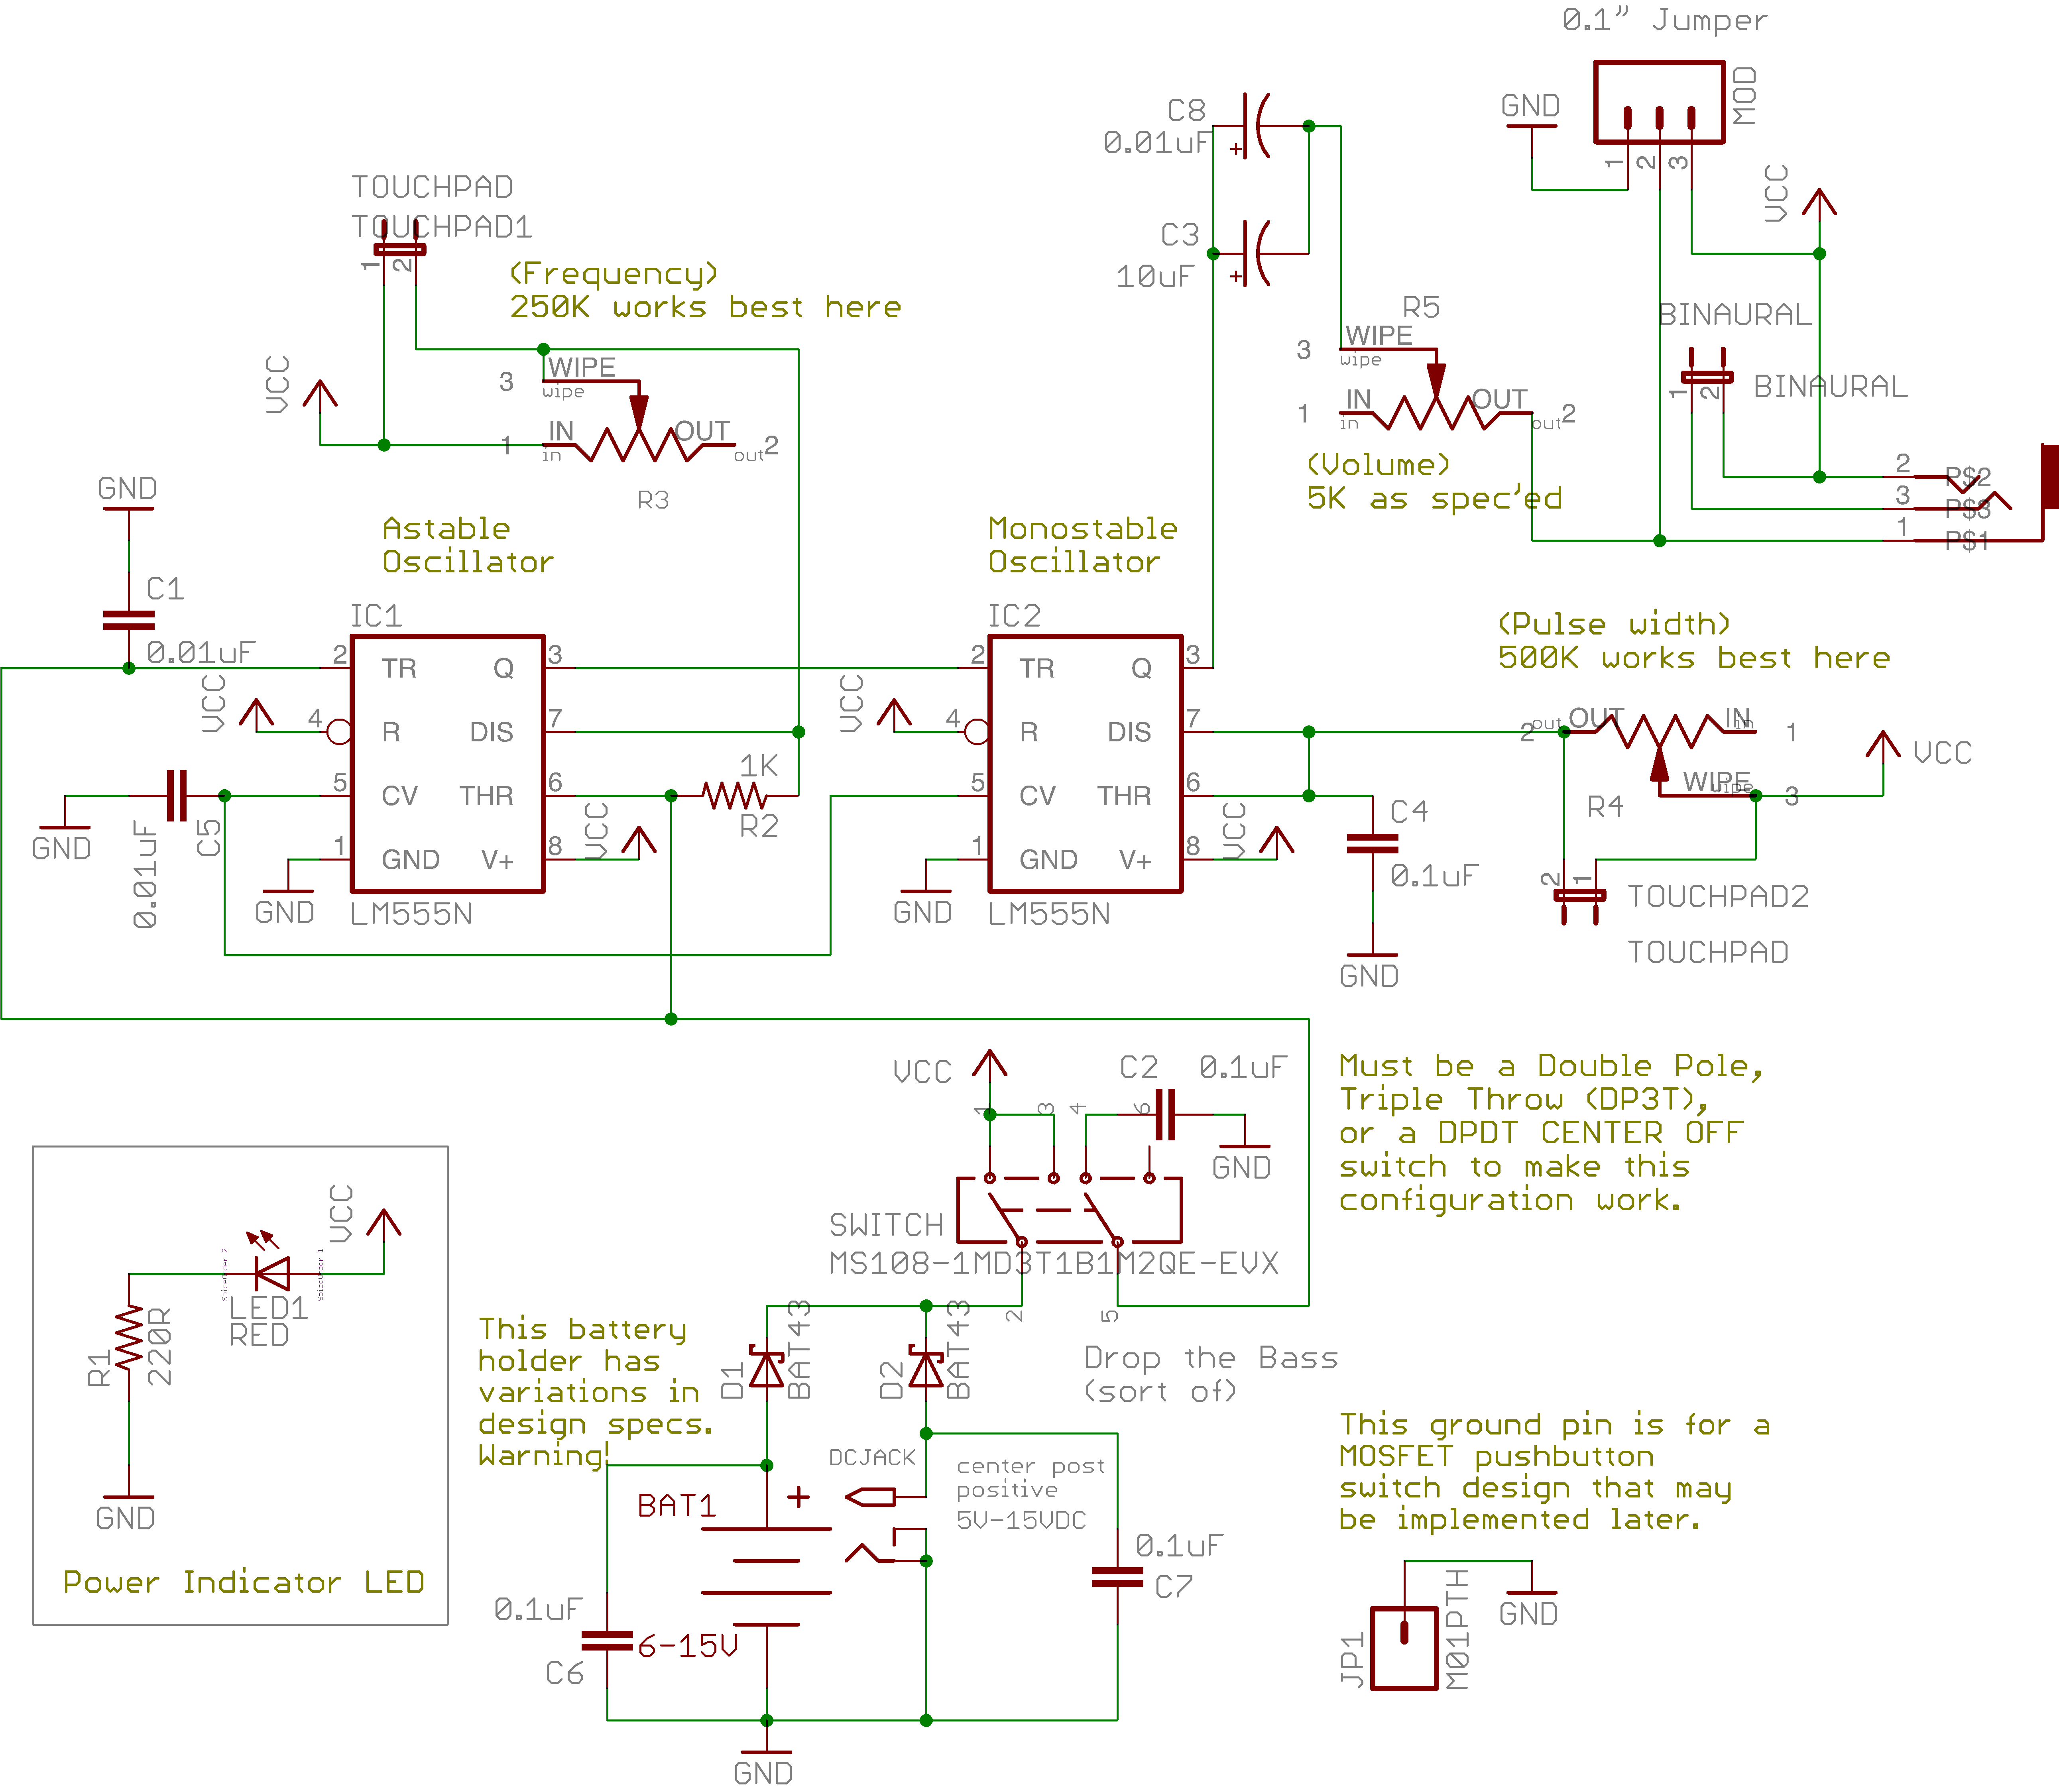
\includegraphics[scale=0.9]{APCschembetter.png} % original file: APCschematic.png
\end{center}
\caption{Schematic, with notes, as implemented in the board for this version.}
\end{figure}

%%%%%%%%%%%%%%%%%%%%%%%%%%%%%%%%%%%%%%%%%%%%%%%%%%%%%%%%%%%%%
%
% Optional section on making the images:
%
%%%%%%%%%%%%%%%%%%%%%%%%%%%%%%%%%%%%%%%%%%%%%%%%%%%%%%%%%%%%%

\ifkey 

\clearpage
\section{How To Make The Images In This Document}

An EagleCAD script is provided in Figure \ref{fig:codelistexport} and in the GitHub repository. Run the script from within EagleCAD and the first set of images will appear. Basically, the script turns on the layers for each particular image, sets color or monochrome, sets the resolution to 600 DPI, and exports each resulting layer set to a PNG file. For instance, before making the \emph{top} layer, the script turns off the set of layers in EagleCAD that would make it hard to parse the top components -- i.e.~all of the ``bottom'' layers, like 16, 22, 24, 26, 28, 30, 32, 34, 36, 40, 42, 52, 122, 126, 128, and, as noted above, 200 (where the logo image silkscreen resides). To make an image of the underside, a similar operation is performed, blanking the ``top" layers. The script writes image files called:

\bigskip

\begin{tabular}{lll}
\tabitem \texttt{fullcolorboard.png} && \tabitem \texttt{boardlayout.png} \\[\sep]
\tabitem \texttt{boardtoplayout.png} && \tabitem \texttt{boardbottomlayout.png} \\[\sep]
\tabitem \texttt{boardbottomsilk.png} && \tabitem \texttt{boardtopsilk.png} \\[\sep]
\tabitem \texttt{boarddimensions.png} \\[\sep]
\end{tabular}

\begin{figure}
\vspace{-0.5in}
% Code listing:
\lstinputlisting[
 language=bash, 
 columns=fullflexible, 
 breaklines=true, 
 basicstyle=\ttfamily\footnotesize, 
 numbers=left, 
 numbersep=5pt,
 commentstyle=\color{mygreen},
 numberstyle=\tiny\ttfamily\color{black}, 
 frame=single]
 {./exportspecificlayers.scr}

\caption{The \texttt{EagleCAD} script to export images from EagleCAD.}
\label{fig:codelistexport}
\end{figure}


The script to appropriately convert the images is seen in Figure \ref{fig:codelistconvert}. The resulting files are called: 

\medskip

\begin{tabular}{lll}
\tabitem \texttt{\colorimagename} && \tabitem \texttt{\twolayermonochrome} \\[\sep]
\tabitem \texttt{\topmonochrome} && \tabitem \texttt{\bottommonochrome} \\[\sep]
\tabitem \texttt{\topsilk} && \tabitem \texttt{\bottomsilk} \\[\sep]
\tabitem \texttt{\boarddimensions} \\[\sep]
\end{tabular}
\medskip

\noindent This script was written for Mac OS X but should run on any system with 
{\color{webblue}\href{https://en.wikipedia.org/wiki/Bash_%28Unix_shell%29}{\texttt{bash}}}
and {\color{webblue}\href{http://www.imagemagick.org/script/index.php}{ImageMagick}} installed.

\newpage

\begin{figure}[ht!]
\vspace{-0.5in}
% Code listing:
\lstinputlisting[
 language=bash, 
 columns=fullflexible, 
 breaklines=true, 
 basicstyle=\ttfamily\footnotesize, 
 numbers=left, 
 numbersep=5pt,
 commentstyle=\color{mygreen},
 numberstyle=\tiny\ttfamily\color{black}, 
 frame=single]
 {./images/imageprep.sh}
\caption{The \texttt{bash} script to correctly color the exported images from EagleCAD.}
\label{fig:codelistconvert}

\end{figure}

\clearpage
\newpage

\subsection{8-bit Art in Eagle CAD}

The PCB also includes three pieces of art from the ancient era of video games. the Asteroids ship was converted using the \texttt{import-bmp.ulp} user language script that is included in Eagle CAD. The other two presented a fun challenge, which was to draw the 8-bit sprites using the Eagle CAD scripting language. It's pretty easy to draw squares and rectangles using the language, so I wrote a Python script that reads in a very simple csv file, composed of rows of comma-separated ``1'' or ``0'' cells. The Python script then writes out a nice (and easily scalable, if you check out the top of the script) Eagle CAD script that draws the figure in the layer you specify. It's much faster than drawing it yourself, and the CAM script runs much faster too, since the sprites are so simple.


\begin{figure}[h!]
\begin{minipage}{3.5in}
% Code listing:
\lstinputlisting[
 language=bash, 
 breaklines=true, 
 basicstyle=\ttfamily\footnotesize, 
 numbers=left, 
 numbersep=5pt,
 commentstyle=\color{mygreen},
 numberstyle=\tiny\ttfamily\color{black}, 
 frame=none]
 {../graphics/pitfallharry.txt}
\end{minipage}
\caption{The comma-separated source text that \texttt{eagledraw.py} uses to draw Pitfall Harry.}
\label{fig:pitfallharry}

\end{figure}


\clearpage
\newpage

\else
	\newpage
\fi


\begin{sidewaystable}
\section*{Bill of Materials}
\begin{footnotesize}
\begin{tabular}{l p{1in} p{1.6in}  p{1.7in}  p{3.0in} }

\large{\textbf{Part}} &  \large{\textbf{Value}} &  \large{\textbf{Device}} &  \large{\textbf{Package}} &  \large{\textbf{Description}} \\[\sep]
\hline\\[\negsep]
BAT1 & 6-15V & BH-9VPC & BH9VPC & These specs, though the battery holder is imprinted with ``BH-9VPC", also match the specs of part number 12BH611-GR. \\
BINAURAL & 0.1\texttt{"} header & JP1E & JP1 & jumper for two-channel audio output. \\
C1  & 0.01$\mu$F & C-EU050-024X044 & C050-024X044 & ceramic disc capacitor  \\
C2  & 0.1$\mu$F & C-EU050-024X044 & C050-024X044 & ceramic disc capacitor   \\
C3  & 10$\mu$F & CPOL-USE2.5-7 & E2,5-7 & polarized capacitor  \\
C4  & 0.1$\mu$F & C-EU050-024X044 & C050-024X044 & ceramic disc capacitor   \\
C5  & 0.01$\mu$F & C-EU050-024X044 & C050-024X044 & ceramic disc capacitor   \\
C6  & 0.1$\mu$F & C-EU050-024X044 & C050-024X044 & ceramic disc capacitor   \\
C7  & 0.1$\mu$F & C-EU050-024X044 & C050-024X044 & ceramic disc capacitor   \\
C8  & 0.01$\mu$F & CPOL-USE2.5-7 & E2,5-7 & polarized capacitor  \\
D1  & BAT43 & DO35-7 & DO35-7 & Schottky diode, 0.45V fwd, 30V, 200mA \\
D2  & BAT43 & DO35-7 & DO35-7 & Schottky diode, 0.45V fwd, 30V, 200mA \\
DCJACK & PJ102A & PJ102A & PJ-102A & DC power jack, 2.0mm center pin, 5.5mm plug \\
IC1 & LM555N & LM555N & DIL08 & 555 Timer IC \\
IC2 & LM555N & LM555N & DIL08 & 555 Timer IC \\
JP1 & M01PTH & M01PTH & 1X01 & 1-pin header to ground \\
LED1 & red & LED ELD260 & 5mm, 2.54mm spacing & Lite-ON 859-LTL2R3KRD-EM, 2mA, 1.8V fwd  \\
LINE & SJ-3523-SMT & SJ-3523-SMT & SJ352 Audio Jack & CUI inc Stereo Audio SMT jack, 3.5mm \\
MOD & 0.1\texttt{"} header & 3 pin header & 1X03 & 3 pin header for mods \\
R1  & 220R & R-US 0207/7 & 0207/7 & through-hole resistor \\
R2  & 1K  & R-US 0207/7 & 0207/7 & through-hole resistor \\
R3  & 250K  & CTS UM296RE series pot & UM296RE POT & Frequency potentiometer \\
R4  & 500K  & CTS UM296RE series pot & UM296RE POT & Pulse-width potentiometer \\
R5  & 5K  & CTS UM296RE series pot & UM296RE POT & Volume potentiometer \\
R6  & 220R & R-US 0207/7 & 0207/7 & through-hole resistor \\
R7  & 220R & R-US 0207/7 & 0207/7 & through-hole resistor \\
SWITCH & MS108-1MD3T1B1M2QE-EVX &  &  & Mountain Switch Toggle DPDT center-off model 108-1MD3T1B1M2QE-EVX \\
TOUCHPAD1 & 0.1\texttt{"} header & JP1E & JP1 & optional touch pad connection \\
TOUCHPAD2 & 0.1\texttt{"} header & JP1E & JP1 & optional touch pad connection \\[\sep]
\hline\\[\negsep]

\end{tabular}
\end{footnotesize}

\end{sidewaystable}

\clearpage

\section{Change Log}

\bd

\+[Revision \revision{}:] February 2017
\bi
\+ Initial release
\+ Changed switch to one in current production
\+ Re-routed and simplified some traces
\+ Moved and added labels
\+ Moved some discrete components
\ei

\+[0.4:] July 2016
\bi
\+ Shrunk the footprint of discrete resistors
\+ Renumbered a few components
\+ Altered the 9V cradle part's footprint to improve pin placement
\+ Changed a few labels
\+ Never released
\ei

\+[0.3:] June 2016
\bi
\+ Changed switch
\+ Moved a few components for clearance
\+ Never released
\ei


\+[0.2:] January 2016
\bi
\+ Revealed a problem with the switch layout
\+ Never released
\ei

\+[0.1:] December 2015
\bi
\+ Corrected problems with component layout, clearance, and part names
\+ Added board cutouts to ensure it only fits in the enclosure in one specific orientation
\+ Shrunk discrete component pin spacings from 10mm to 7mm
\+ Never released
\ei
\ed

\vfill

\begin{center}
\emph{This is the last page.}
\end{center}

\end{document}

